\setcitestyle{numbers,open={[},close={]}}

Having developed a method and the means to implement it, we now apply it to a number of cases of lithium materials.   We choose three common lithium compounds with a variety of properties; metallic lithium, ionic LiF, and covalent $\mathrm{Li_2O}$.  We also analyze a mixed compound obtained after observing beam damage on LiF during a transformation into metallic lithium, which we will also discuss.  

Before discussing specific cases, it should be noted that all calculations were run in a manner to account for the peculiarities of lithium in DFT. In particular, atomic sphere radii on the lithium were maximized to minimize core leakage and monopole effects were verified to be negligible.  The standard DFT convergence tests (K points, RKMax) were also performed and all cells were relaxed according to volume.  All supercells were performed in \textit{P1} symmetry so as to only produce a single core hole atom per cell.  

All of the experimental results were obtained at McGill on a Hitachi SU900 TE-SEM.  Spectra were acquired at 30 keV to minimize the beam damage to the lithium.  All spectra had their backgrounds removed through a power law fit (see Section \ref{bg_section}) and were deconvoluted using the Richardson-Lucy algorithm (also Section \ref{deconvolution}).

\section{Lithium Oxide}

We begin by investigating $ \mathrm{Li_2O} $. Screening calculations were performed as described in Section \ref{implementation}.   After the initial two calculations, (with no hole then full hole), the density around the excited lithium atom was plotted, see Fig \ref{Li2O_contour}.  

\begin{figure}
	\centering
	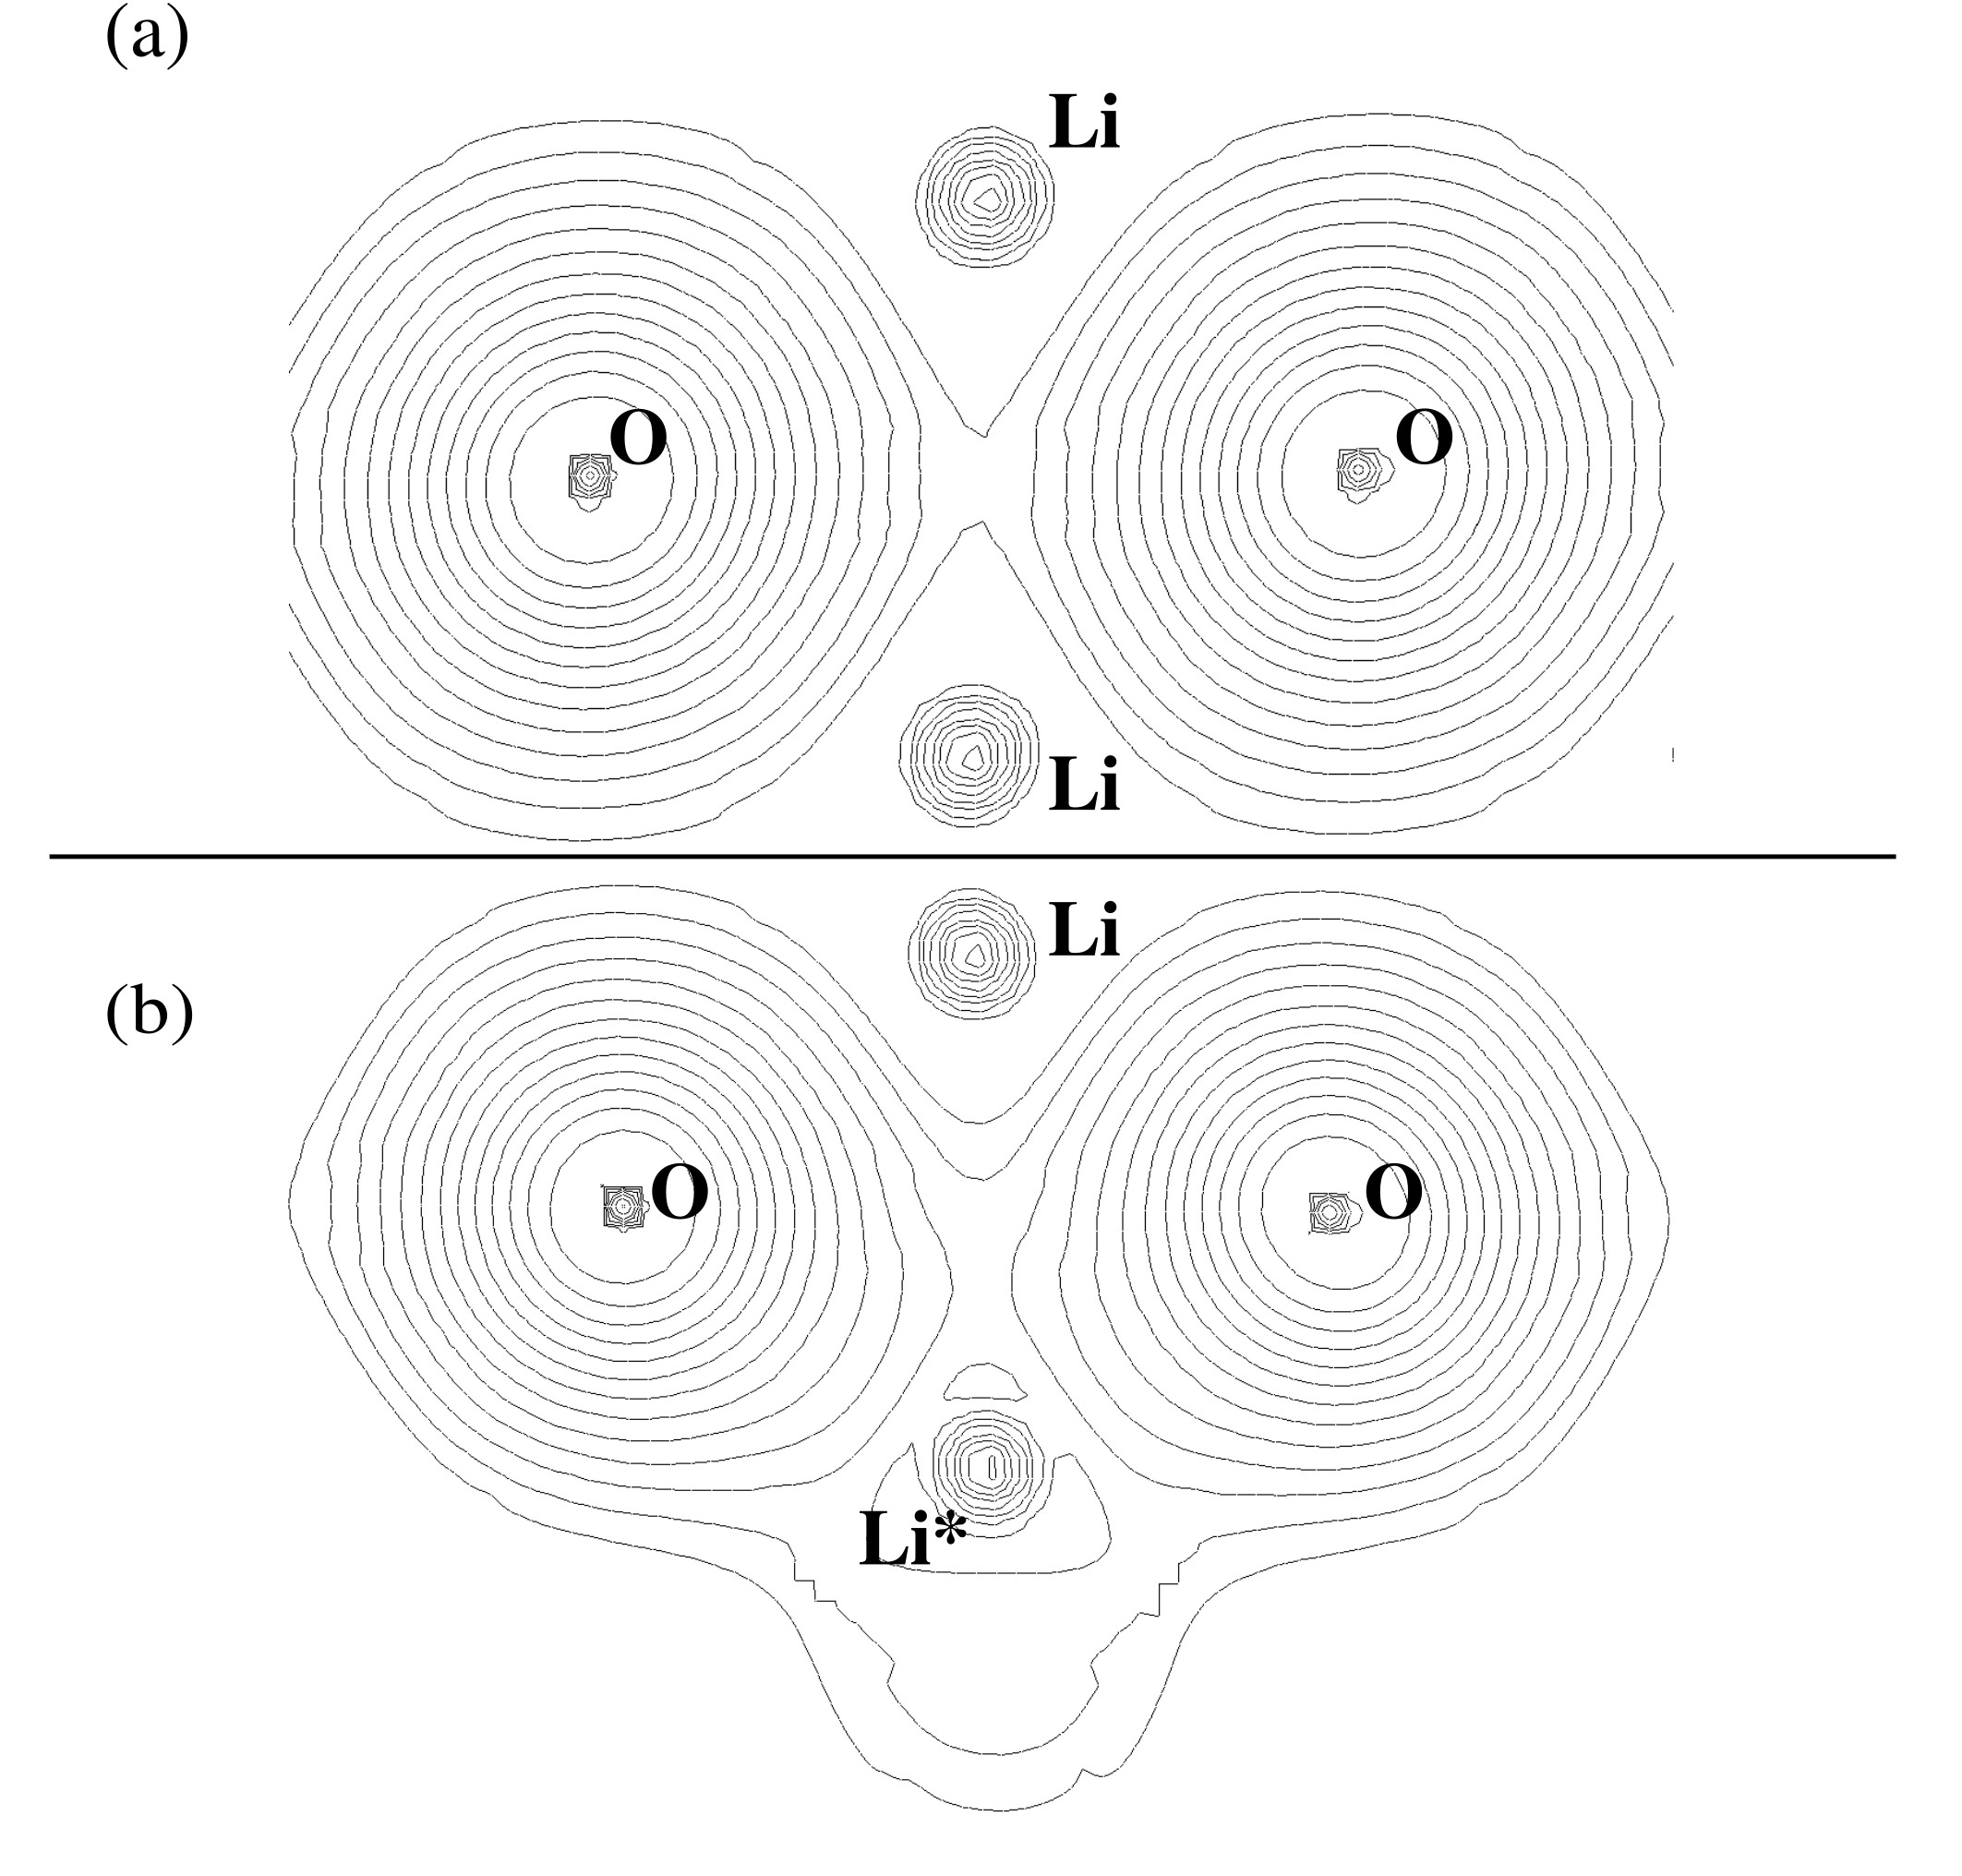
\includegraphics[scale=0.15]{Li2Ocontour_plot}
	\caption{Effect of introducing a core hole in $ \mathrm{Li2O} $.  (a) no hole crystal.  (b) Crystal with hole on starred lithium atom, inducing a response from the valence electrons.  Contour lines on a logarithmic scale. }
	\label{Li2O_contour}
\end{figure}

The density plots clearly show valence electrons in the material being attracted to the excited atom. This indicates that the core hole should have both a noticeable effect on the final states and that it is screened as well.  We can also see that even the closest lithium atom is largely unaffected by the core hole, in agreement with the supercell size being sufficient to isolate core holes.  Calculating the difference in electron occupancy shows a decrease of 0.88 electron in the basin.  This decrease is smaller then would be expected the no screening limit and according to Eq \ref{final_eq}, indicates that the hole is 12\% screened.  A third calculation was then performed using a decreased hole size to obtain a final spectra.  The ELNES K edge from all three simulations are compared to experiment in Fig \ref{Li2O_three}.  

From the comparison to experiment, we can observe that the full hole provides good agreement, as previously predicted in the literature \cite{mauchamp_ab_2006}. However, the screened hole provides a superior result, which can be emphasized by considering the ratio of the two peaks at $\sim$55eV and $\sim$58 eV.  Quantitatively comparing the values, presented in Table \ref{ratio}, reveals a dramatic improvement, decreasing the error from 20\% to  6\%.  The qualitative and quantitative improvements to the results support the validity of the new method and highlights it's necessity.  

\begin{table}
	\centering
	\begin{tabular}{ccc}
		& Ratio & Error \\
		\hline
		Experiment & 0.71 & -  \\
		Full Hole & 0.85 & 20\%  \\
		Screened Hole & 0.66 & 6\%  \\
		
	\end{tabular}
	\caption{The ratio of intensities in the $\mathrm{Li_2O}$ spectra between the two peaks at 55 eV and 58 eV.  Errors were calculated relative to experiment.   }
	\label{ratio}
\end{table}




\begin{figure}
	\centering
	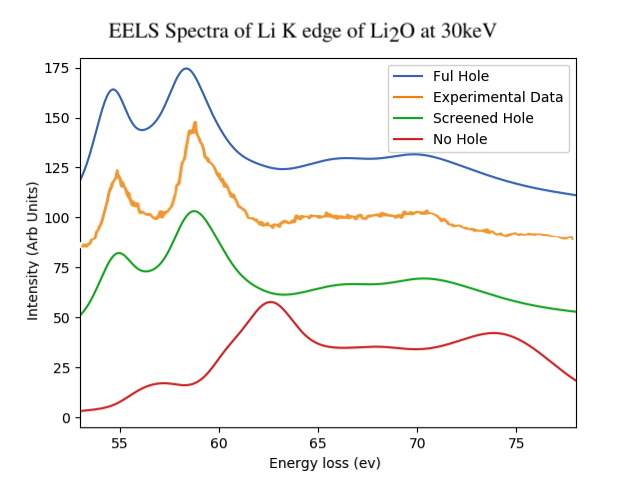
\includegraphics[scale=0.45]{Li2O_three}
	\caption{Lithium K edge of $ \mathrm{Li_2O} $ from the three calculations taken with varying degrees of core hole. }
	\label{Li2O_three}
\end{figure}

\section{Lithium}
We now shift our attention to metallic lithium, which has previously presented a  number of challenges to experimental analysis.  As a metal, it has been predicted to exhibit no core hole effects due to valence screening, and a density plot reveals that core  holes have a large impact on the electron density, see Fig \ref{Li_countours}, supporting the notion that the hole may indeed be entirely screened.  The excited atom attracts a number of valence electrons and  distorts the electron clouds of the surrounding atoms more aggressively than in $ \mathrm{Li_2O} $.  Calculating the screening factor however reveals that the lithium core hole is in reality only $ \sim$41\% screened.  A comparison with experimental spectra confirms this fact, Fig \ref{Li_spectra}.


\begin{figure}
	\centering
	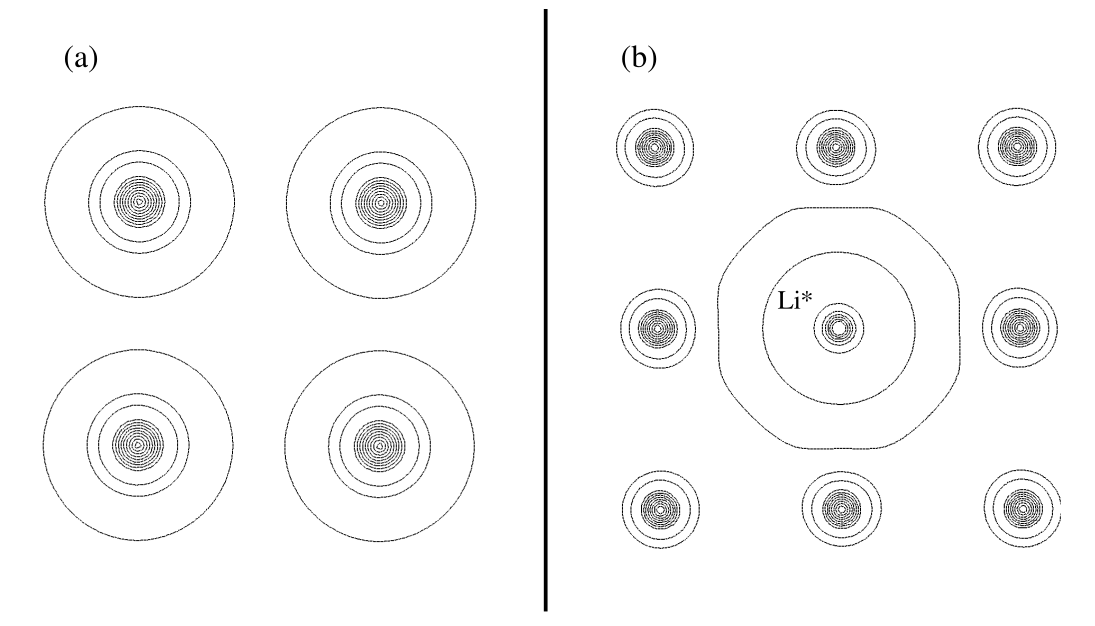
\includegraphics[scale=0.4]{Li_contours}
	\caption{Electron density map of metallic lithium, before (a) and after (b) introduction of a core hole on the starred atom.  The contours are on equal logarithmic scales.}
	\label{Li_countours}
\end{figure}




\begin{figure}
	\centering
	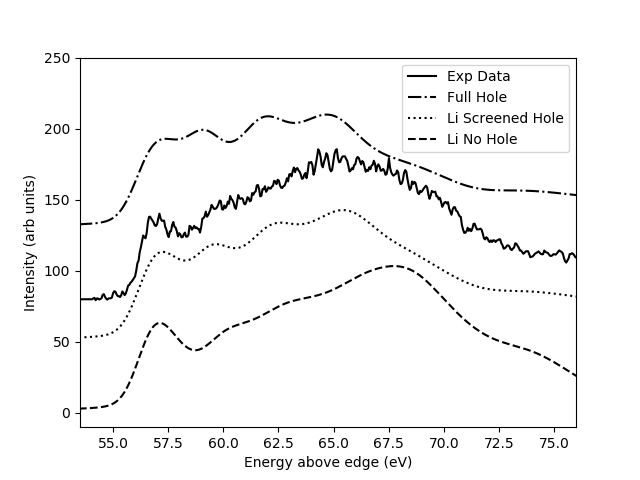
\includegraphics[scale=0.45]{Li}
	\caption{Lithium K edge of Li from the three calculations taken with varying degrees of core hole. }
	\label{Li_spectra}
\end{figure}


Again, the literature result assuming no hole provides better agreement than the full hole, but is inferior to the screened hole result.  Of particular note is the small peak located at $ \sim$58 eV, which is underestimated, in the no hole spectra, overestimated in the full hole, and correctly accounted for in the screened case.  The only moderate (41\%) screening goes against common convention in the literature that metals do not exhibit core hole effects.  A couple of more extreme cases have been highlighted  (Cu, Al?), but the slight yet significant improvements observed with lithium suggest that screened core holes should be included or at least calculated in all cases.  It should be noted that lithium's lack of core electron screening may also contribute to the large core hole effects, which could be lessened for heavier elements. 

\section{LiF}
We continue our investigation of pure molecules by considering LiF.  LiF has been one of the more published EELS results for lithium and simulations have obtained good agreement with a full core hole approximation \cite{mauchamp_ab_2006}.  We again begin with a qualitative probe of the electron density, see Fig \ref{LiF_countours}.  We can see that the introduction of a hole has minor effects on the electron density, but these are largely limited to slight distortions in the fluorine electron cloud, see Fig \ref{LiF_countours}. Additionally, despite the loss of a core electron, the density around the excited lithium atom retains much of its initial form. The minimal effect of introducing a core is reflective of fluorine's high electronegativity which ``freezes" all of the electrons in place and minimizes any kind of valence electron screening.  This effect is confirmed by calculating the screening coefficient which was determined to be zero in this case. Consequently, LiF represents the no screening case of Eqn. \ref{density_calc} and we can take the full hole spectra as the final spectrum.  Plotting the spectra against experiment confirms that a full hole does indeed produce good agreement, Fig \ref{LiF_spectra}.  The lack of screening in LiF also explains the good results obtained in literature when using only a full hole.  It also supports the theory that inserting a full hole is sufficient in the case of strong insulators, although again, lithium's lack of core screening limit the generality of that statement.  

\begin{figure}
	\centering
	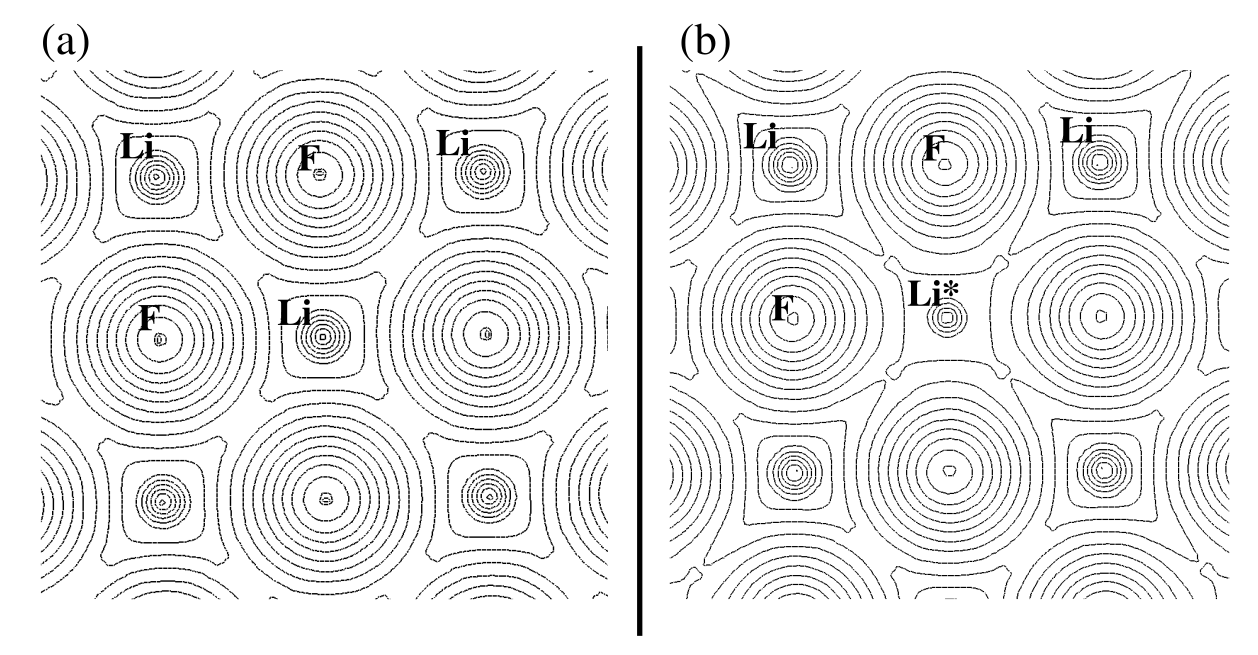
\includegraphics[scale=0.35]{LiF_countours}
	\caption{Electron density map of LiF, before (a) and after (b) introduction of a core hole on the starred atom.  The contours are on equal logarithmic scales.}
	\label{LiF_countours}
\end{figure}

\begin{figure}
	\centering
	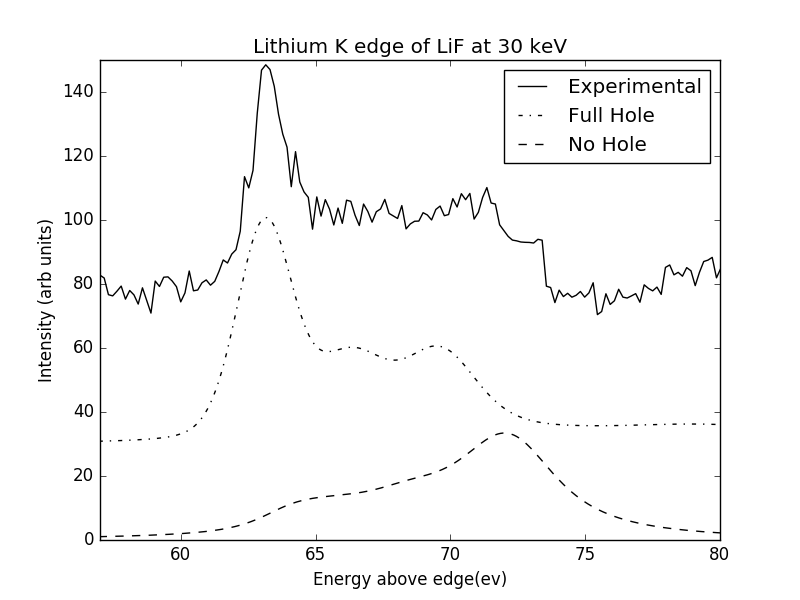
\includegraphics[scale=0.45]{LiF_spectra}
	\caption{Lithium K edge of LiF from the two calculations taken with varying degrees of core hole. }
	\label{LiF_spectra}
\end{figure}



\section{Li-LiF Mixture}
We will conclude the results section with a case that demonstrates the full importance of accounting for screening in ELNES calculations.  When obtaining the spectra for LiF, we observed a transformation to metallic lithium, due to the beam damage.   During this transformation, an intermediate spectra was acquired.  To investigate the transformation, a linear combination of the spectra from metallic lithium and LiF was compared to the experimental result, see Fig \ref{mix-screened}.  The good agreement obtained here supports both the inclusion of screening and that the sample contains  Li, LiF, and no intermediate phases or contamination.  The importance of screening is highlighted in Fig \ref{mix-unscreened}, where the no hole lithium spectra is used, resulting in a poorer fit, that fails to reproduce the peak at 59eV.  This unaccounted for peak would prevent such an  analysis from confirming the purity of the sample and of the mixture.  



\begin{figure}
	\centering
	\begin{subfigure}{0.45\textwidth}
		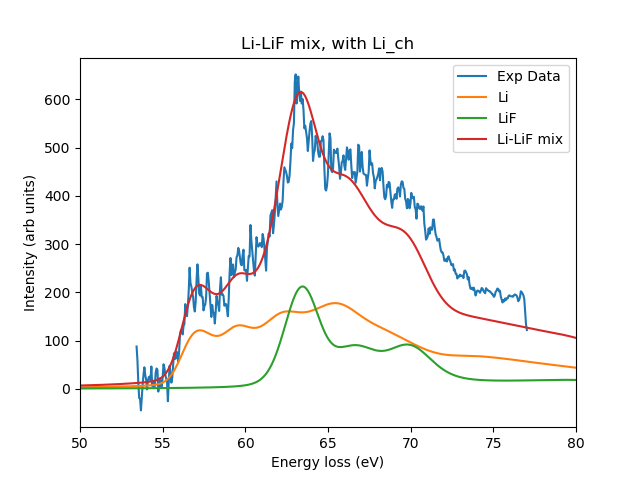
\includegraphics[scale=0.5]{Li-LiF_mix_screened}
		\caption{}
		\label{mix-screened}
	\end{subfigure}
\hfill
	\begin{subfigure}{0.45\textwidth}
		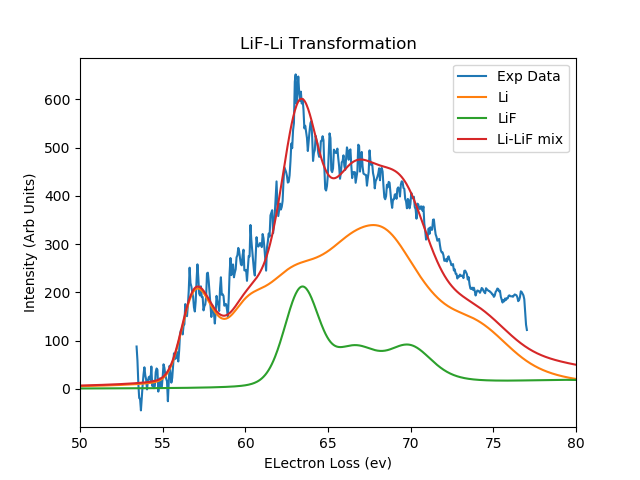
\includegraphics[scale=0.5]{Li-LiF_mix_no-screen}
		\caption{}
		\label{mix-unscreened}
	\end{subfigure}
	\caption{Lithium K edge of Li-LiF mix using full hole LiF spectrum and screened (a) and unscreened (b) Li spectrum. }

\label{Li-LiF_mix_screened}
\end{figure}



\section{Discussion}
The cases handled here highlight the importance of including a core hole and calculating screening effects when performing ELNES on lithium.  In every case, a core hole was necessary, including metallic lithium which had been predicted to not exhibit core hole effects.  Additionally, in every case except LiF, screening was non negligible and the first order method developed in Chapter \ref{methods} result in dramatic improvements to experimental agreement.  The impact of including screening in ELNES calculations is made more apparent when dealing with unknown cases such as the Li-LiF mixture where it was essential to fingerprinting the near edge structure.  The improvement to the peak ratio in $ \mathrm{Li2O} $ is another key feature in terms of identifying oxidation on lithium edges, or taking the steps to quantitative analysis.  Finally the reliable agreement between calculation and experiment help solidify the validity of the technique of performing EELS at 30keV to analyze beam sensitive materials, a result with considerably less weight without excellent agreement between the results.  





